\documentclass{article}
\usepackage{tikz}
\usetikzlibrary{positioning}
\usetikzlibrary{shapes.geometric}
\usetikzlibrary{shapes.symbols}
\usetikzlibrary{shadows}
\usetikzlibrary{arrows}

\pagestyle{empty}

\def\rbell{0.3}
\def\drawcol{darkgray}
\def\fillcol{gray!20!white}
\newcommand{\queen}[2]{ 
	\begin{scope}[shift={#2}]
	\draw [very thick,darkgray,fill=\fillcol,#1]
	% contour
    (0,1) .. controls +(1,-1) and +(-1,-1) .. ++(6,0) 
			-- ++(-0.5, 1) -- ++(0.5,1)
			-- ++(0.75, 3) arc (-120:240:\rbell) -- ++(-1.25,-1)
			-- ++(-0.7, 3) arc (-100:260:\rbell) -- ++(-0.9, -2)
			-- ++(-0.9, 2.5) arc(-90:270:\rbell) -- ++(-0.9, -2.5)
			-- ++(-0.9, 2) arc (-80:280:\rbell) -- ++(-0.7, -3)
			-- ++(-1.25, 1) arc (-60:300:\rbell) -- ++(0.75, -3) 
			-- ++(0.5, -1) -- cycle;
	\draw [thin,\drawcol,#1] (0.5, 2) .. controls +(1,-1) and +(-1, -1) .. +(5,0);
	\draw [thin,\drawcol,#1] (0, 3) .. controls +(1,-1) and +(-1, -1) .. +(6,0);
	\draw [semithick,\drawcol,#1] (1, 4.5) .. controls +(1.25, 1.25) and +(-1.25, 1.25)
										.. +(4, 0);
	\end{scope}}

\newcommand{\board}[2] {
	\begin{scope}[shift={#2}]
		\begin{scope}[scale={#1}]
			\draw[fill=brown!5!white,draw=brown,very thick] (0,0) rectangle (8,8);
			\foreach \x in {0, 2, 4, 6}
				\foreach \y in {0, 2, 4, 6} {
					\draw[fill=brown!70!white] (\x, \y) rectangle +(1,1);
					\draw[fill=brown!70!white] (\x+1, \y+1) rectangle +(1,1);}
		\end{scope}
	\end{scope}}

\newcommand{\queens}[3]{
	\begin{scope}[shift={#1}]
		\foreach \x/\y in {#2} {\queen {#3} {(10*\x+2,10*\y+1)}}
	\end{scope}}

\newcommand{\position}[3]{
	\board {10} {#1}
	\queens {#1} {#2} {#3}}


\begin{document}

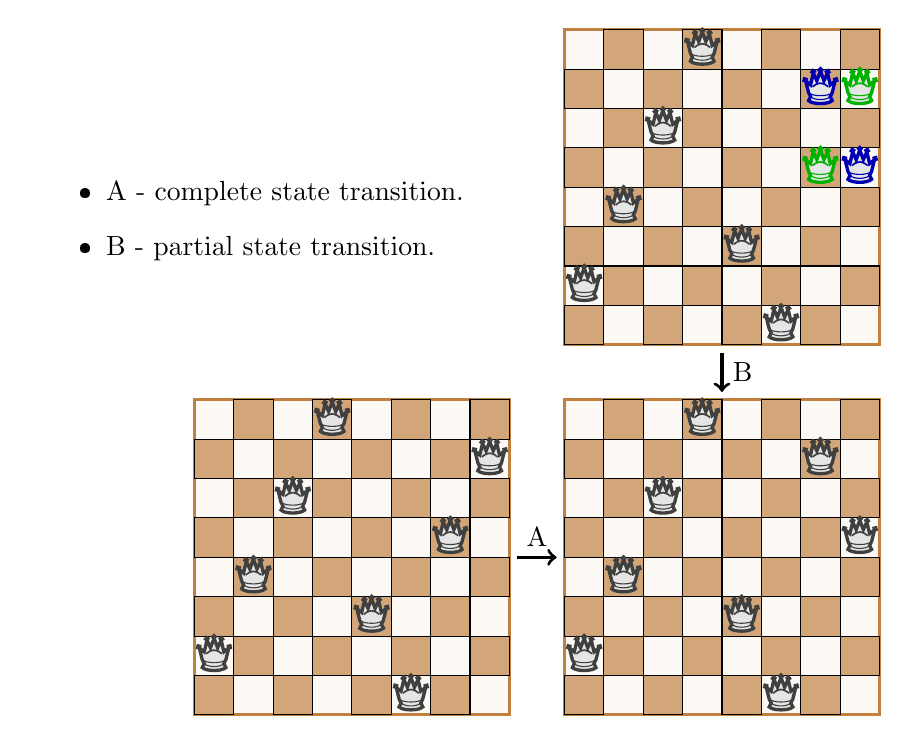
\begin{tikzpicture}
\node [text width=6.0cm] at (1.0, 6.5) {
\begin{itemize}
\item A - complete state transition.
\item B - partial state transition.
\end{itemize}};
\begin{scope}[scale=0.05]
% complete state 
\position {(0,0)} {0/1,1/3,2/5,3/7,4/2,5/0,6/4,7/6} {}
\position {(94,0)} {0/1,1/3,2/5,3/7,4/2,5/0,6/6,7/4} {}
\draw[->,very thick] (82,40)-- node [midway,above] {A} (92,40);
% partial state
\position {(94,94)} {0/1,1/3,2/5,3/7,4/2,5/0} {}
\queens {(94,94)} {6/4,7/6} {draw=black!30!green}
\queens {(94,94)} {6/6,7/4} {draw=black!30!blue}
\draw[->,very thick] (134,92) -- node[midway,right] {B} (134,82);
\end{scope}
\end{tikzpicture}
\end{document}

